\input parameters.tex
%\begin{abstract}
%This document is a model and instructions for \LaTeX.
%This and the IEEEtran.cls file define the components of your paper [title, text, heads, etc.]. *CRITICAL: Do Not Use Symbols, Special Characters, Footnotes, 
%or Math in Paper Title or Abstract.
%\end{abstract}
%
%\begin{IEEEkeywords}
%component, formatting, style, styling, insert
%\end{IEEEkeywords}

\section{Overview}
Our final project aims to solve a large-scale non-convex QCQP problem with the Hessian matrix to be \emph{sparse} and \emph{negative definite}. In this report we consider a distributed method for solving this QCQP problems called \emph{Alternating Direction Method of Multipliers} (ADMM). The results show that our implementation is able to correctly solve really large problems with a million dimensional QCQP problems.

\section{Problem Formulation}
The problem we wish to solve is
\[
\begin{array}{ll}
\min&f(x,y):=\frac{1}{2}(\bm x\trans\bm A\bm x+\bm y\trans\bm A\bm y)-\bm b\trans\bm x-\bm c\trans\bm y\\
\mbox{s.t.}&h_1(\bm x,\bm y)=\frac{1}{2}(\bm x\trans\bm x-1)=0\\
&h_2(\bm x,\bm y)=\frac{1}{2}(\bm y\trans\bm y-1)=0\\
&h_3(\bm x,\bm y)=\bm x\trans\bm y=0,
\end{array}
\]
where $\bm x,\bm y\in\mathbb{R}^n$ are the optimization variables. The terms $\bm A,\bm b,\bm c$ refer to the problem data. We further require that $\bm A$ to be sparse and negative definite.

Following the similar idea of ADMM [1], we consider solving the quadratic penalized version of the original problem:
\begin{equation}
\begin{array}{ll}
\min&f(x,y)+\lambda_3(\bm x\trans\bm y)+\frac{\rho}{2}\|\bm x\trans\bm y\|_2^2
\\
\mbox{such that}&\frac{1}{2}(\bm x\trans\bm x-1)=0\\
&\frac{1}{2}(\bm y\trans\bm y-1)=0,
\end{array}
\end{equation}
where $\rho$ is a penalty parameter and $\lambda_3$ refers to the \emph{Lagrange multiplier} for the third constraint $h_3(\bm x,\bm y)$. We can formulate an iteration for solving this problem:
\begin{subequations}
\begin{align}
\bm x^{k+1}&=\arg\min_{\|\bm x\|=1}\frac{1}{2}\bm x\trans\bm A\bm x-\bm b\trans\bm x+\lambda_3^k(\bm x\trans\bm y^k)+\frac{\rho}{2}\|\bm x\trans\bm y^k\|_2^2\label{Eq:2:a}\\
\bm y^{k+1}&=
\arg\min_{\|\bm y\|=1}\frac{1}{2}\bm y\trans\bm A\bm y-\bm c\trans\bm y+\lambda_3^k(\bm y\trans\bm x^{k+1})\label{Eq:2:b}\\
&\qquad\qquad\qquad\qquad\qquad\qquad\qquad\qquad+\frac{\rho}{2}\|\bm y\trans\bm x^{k+1}\|_2^2\nonumber\\
\lambda_3^{k+1}&=\lambda_3^k+\rho((\bm x^{k+1})\trans\bm y^{k+1})\label{Eq:2:c}\\
\lambda_1^{k+1}&=-(\bm x^{k+1})\trans\bm A\bm x+(\bm x^{k+1})\trans\bm b\nonumber\\
\lambda_2^{k+1}&=-(\bm y^{k+1})\trans\bm A\bm y+(\bm y^{k+1})\trans\bm c\nonumber
\end{align}
\end{subequations}
where $\bm x^k,\bm y^k$ are the $k$th iterate of the variables above, and the update rule for $\lambda_i$ (associated for the constraint $h_i(\bm x,\bm y)=0$) follows from the KKT condition. Here the stopping criteria is decided by the instructor:
\[
\max\left\{
\frac{\|\nabla_{\bm x}L(\bm x,\bm y,\bm\lambda)\|}{1+\|\bm b\|},
\frac{\|\nabla_{\bm y}L(\bm x,\bm y,\bm\lambda)\|}{1+\|\bm c\|},
\|h(\bm x,\bm y)\|
\right\}\le\mbox{tol}.
\]
where $L(\bm x,\bm y,\bm\lambda)$ refers to the \emph{Augmented Lagrangian function} for the original problem.

The update rules (\ref{Eq:2:a}) and (\ref{Eq:2:b}) are equivalent to solve \emph{trust-region subproblems} (TRS). As a result, the main computational challenge for this project is to solve the TRS.

\section{Solving for the Trust-Region Subproblem}
The subproblem for solving (\ref{Eq:2:a}) and (\ref{Eq:2:b}) is to
\begin{equation}\label{Eq:3}
\begin{array}{ll}
\min_{\|\bm p\|=1}&\bm p\trans\bm Q\bm p+\bm g\trans\bm p
\end{array}
\end{equation}
where $\bm p\in\mathbb{R}^n$ is the optimization variable, $\bm Q\in\mathbb{R}^{n\times n}$ are symmetric. To guarantee both the convergence and reasonable running time of ADMM algorithm, we are required to find the exact global minimum to (\ref{Eq:3}) in super-short time. Standard methods for solving the problem (\ref{Eq:3}) exactly require either \emph{factorization} or \emph{inversion} of the matrix $\bm Q$. However, the cost of these operations scales poorly with the problem dimensionality. It is therefore of interest to explore the matrix-free methods guaranteed to solve (\ref{Eq:3}) efficientlly.

Recently, a generalized eigenvalue characterisation for TRS is derived in [2] via solving a \emph{single} generalized eigenvalue problem (GEP). This algorithm is shown to be extremely efficient for solving the TRS. In this project we extend this result by making use of the special structure of our specific problem setting.

\subsection{Theoretical results}\label{sub:A}
In this sub-section, we show that how the optimal solution for a so-called \emph{easy case} TRS can be obtained, and argue that it suffices only to deal with the easy case for this project setting.
\begin{thm}
(From Theorem (3.3) in [2])
The optimal Lagrange multiplier (associated with the optimal solution to (\ref{Eq:3})) is the \textbf{largest real eigenvalue} $\lambda^*$ of the $2n\times 2n$ matrix pencil $\bm M_0+\lambda\bm M_1$, where
\begin{subequations}
\begin{equation}\label{Eq:4:a}
\begin{array}{ll}
\bm M_0=\begin{pmatrix}
-\bm I_{n}&\bm Q\\\bm Q&-\bm g\bm g\trans
\end{pmatrix},
&
\bm M_1=\begin{pmatrix}
\bm0_{n}&\bm I_n\\
\bm I_n&\bm0_n
\end{pmatrix}
\end{array}
\end{equation}
Moreover, suppose the corresponding eigenvector for $\lambda^*$ is 
$\begin{pmatrix}
y_1\\y_2
\end{pmatrix}_{2n\times 1}$. 
If $\bm g\trans\bm y_2\ne0$ (easy case), then a global optimal solution $\bm p^*$ is obtained by:
\begin{equation}
\bm p^*=-\mbox{sign}(\bm g\trans\bm y_2)\frac{\bm y_1}{\|\bm y_1\|}
\end{equation}
\end{subequations}
\end{thm}

In our project setting, the vector $\bm g$ is randomly generated.  When $\bm g\trans\bm y_2=0$ holds, then from proposition (4.1) in [2], we imply $\bm y_1=\bm0$. Or equivalently $\bm B\trans\bm B\bm y_2=\lambda^*\bm y_2$. Therefore, the hard case will occur only when the randomly generated vector $\bm g$ belongs to the set $\mathcal{N}(\bm B\trans\bm B-\lambda^*\bm I)^\perp$, where $\dim((\bm B\trans\bm B-\lambda^*\bm I)^\perp)=n-1$. Since \emph{the probability for which the vector drawn randomly from $\mathbb{R}^n$ lies in a set with dimension $n-1$ is zero}, it makes no difference to assume that all TRS we aim to solve are the \emph{easy case}. 

\section{Practical Implementation}

The algorithm of the TRS solver described in subsection~(\ref{sub:A}) is summarized as follows:

\begin{algorithm}
    \SetKwInOut{Input}{Input}
    \SetKwInOut{Output}{Output}

    %\underline{function Euclid} $(a,b)$\;
    \Input{Problem Data $\bm Q,\bm g$}
    \Output{global minimum to the TRS (\ref{Eq:3})}
    Compute the rightmost eigenvalue $\lambda^*$ of $\bm M_0+\lambda\bm M_1$,  and an eigenvalue $\begin{pmatrix}
y_1\\y_2
\end{pmatrix}$ such that 
$
\qquad\bm M_0\begin{pmatrix}
y_1\\y_2
\end{pmatrix}=-\lambda\bm M_1\begin{pmatrix}
y_1\\y_2
\end{pmatrix}
$\;
    {
    Obtain the global minimum by computing $\bm p^*=-\mbox{sign}(\bm g\trans\bm y_2)\frac{\bm y_1}{\|\bm y_1\|}$\;
    }
      {
        return $\bm p^*$\;
      }
    \caption{Solve the TRS (\ref{Eq:3})}
\end{algorithm}
\paragraph{Remark 1}

In general, the dominant computation cost in solving the TRS is for solving the GEP. We use the MATLAB command $\texttt{eigs}$ instead of $\texttt{eig}$~, considering the large-scale of $\bm M_0$ and $\bm M_1$. Specifically, the code for solving the GEP should be
\begin{verbatim}
[v,~] = eigs(@(x)MM0timesx1(c,x,rho,A,p),...
              2*n,-MM1,1,'lm',OPTS);
\end{verbatim}
where $\texttt{MM0timesx1(x)}$ is a function handle that computes the matrix-vector multiplication $\bm M_0\bm x$. This method takes the advantage of the special structure of $\bm M_0$ and $\bm Q$ to \emph{accelerate the algorithm}, and \emph{saves memory} over storing the large-scale matrix $\bm M_0$.
\paragraph{Remark 2}

Moreover, our solver makes use of the eigenvector $[y_1;y_2]$ from the previous iteration as the initial guess for the eigenvalue problem in the next iteration, in order to achieve fast convergence.

\paragraph{Remark 3}

After some experiments, we find that this GEP can be solved quickly under the \emph{Krylov subspace} with dimension $p=5$. Thus we set the maximum size of Krylov subspace to be 5 for the \texttt{eigs} solver.


\paragraph{Remark 4}
As suggested in [3], we enlarge the dual step size for updating the multiplier $\lambda_3$ from $1$ to $1.95$ to acclerate convergence. In this setting we can see that our algorithm achieves at least global linear convergence, which confirms the result shown in [3] as well.

\paragraph{Remark 5}
We assume that the penalty parameter $\rho$ should grow linearly with the norm of $\bm b$ divided by the size of $\bm A$. Over some experiments, we set the relation to be 
\[
\rho \cong 10.75\times\frac{\|\bm b\|_2}{\|\bm A\|_F}
\]
\paragraph{Remark 6}
We find that the update formula of dual variable (\ref{Eq:2:c}) is not the dominant cost, and therefore at each iteration we update this dual variable exactly after updating $\bm x$ (\ref{Eq:2:a}) or $\bm y$ (\ref{Eq:2:b}) to accelerate the covergence.

\paragraph{Remark 7}
When the norm $\|\bm b\|$ and $\|\bm c\|$ is small, we choose the initial guess to be the solution to the \emph{eigenvalue problem}
\[
\begin{array}{ll}
\min_{\|\bm x\|=1,\|\bm y\|=1}&\frac{1}{2}(\bm x\trans\bm A\bm x+\bm y\trans\bm A\bm y)\\
\end{array}
\]
Otherwise, we choose the initial guess for $\bm y$ to be $\bm c$ to minimize the affine term $-\bm c\trans\bm y$.

Here we present parital of our experiment results in Fig~(\ref{fig:11}). For details you may refer to the appendix.
\begin{figure}
\centering\caption{Running Results for $s=1$}
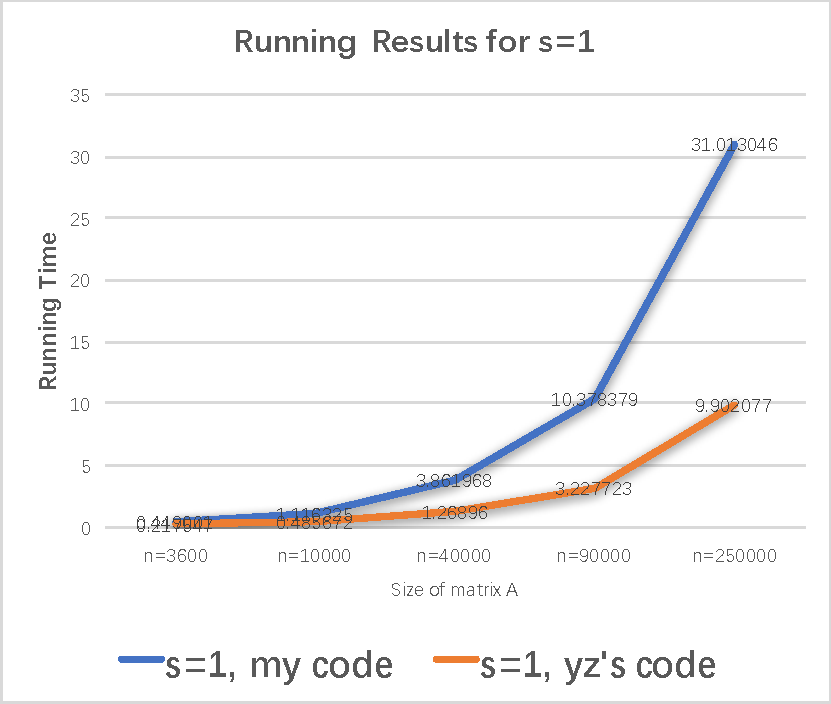
\includegraphics[page=1,width=6cm]{P_4.pdf}
\label{fig:11}
\end{figure}

\section{Conclusion}
As we can see, the running time for our algorithm is roughly three times of that for instructor's. The main computation cost is the generalized eigenvalue solver. When computing a relatively large scale rightmost eigenvalues, the performance of MATLAB solver \texttt{eigs} is not so satisfying. My conjucture is that perhaps the idea for the \emph{augmented Rayleigh-Ritz percedure} described in [4] can be extended into this problem, which looks promising. Due to the limited time, I don't have time to realize this idea. In the future I will think about it and discuss some ideas with the instructor. 
\medskip
 
\begin{thebibliography}{9}
\bibitem{ML}
Stephen Boyd $\&$ Neal Parikh $\&$ Eric Chu $\&$ Borja Peleato $\&$ Jonathan Eckstein (2011)
\textit{
Distributed Optimization and Statistical Learning via the Alternating Direction Method of Multipliers
}
foundations and Trends in Machine Learning, 3,
1-122.
\bibitem{latexcompanion} 
Adachi, S., Iwata, S., Nakatsukasa, Y., $\&$ Takeda, A. (2017). 
\textit{
Solving the Trust-Region Subproblem By a Generalized Eigenvalue Problem
}. SIAM Journal on Optimization, 27, 269-291.

\bibitem{admm}
Guo, K $\&$ Han, D.R. $\&$ Wu, Ting-Ting. (2017). 
\textit{
Convergence of alternating direction method for minimizing sum of two nonconvex functions with linear constraints
}. International Journal of Computer Mathematics. 94. 1653-1669.
\bibitem{yz}
Wen, Zaiwen $\&$ Zhang, Yin. (2017). 
\textit{
Accelerating Convergence by Augmented Rayleigh--Ritz Projections For Large-Scale Eigenpair Computation}. 
SIAM Journal on Matrix Analysis and Applications. 38. 273-296.
\end{thebibliography}













\end{document}